\documentclass[usletter]{article}
\usepackage{graphicx}
\usepackage{amsfonts}
\usepackage{amsthm}
\usepackage{amsmath}
\usepackage{scribe}
\usepackage[margin=1.5in]{geometry}
\usepackage{algorithm}
\usepackage{algorithmicx}
\usepackage{float}
\usepackage[noend]{algpseudocode}

\begin{document}

\makeheader{Minsheng Zhang}                              % your name
           {March 01, 2015}                          % lecture date
           {7}                                       % lecture number
           {NP-complete}  % lecture title

\noindent
In this week, we discuss that independent set problem and coloring a graph are NP-complete problems by reducing 3SAT to them. 

\section{3SAT $\rightarrow$ Independent Set}
First, we prove that independent set is an NPC problem by reducint 3SAT to it.

Independent set problem: Given a graph G = (V,E), an independent set is a set of vertices S $\subseteq$  V such that if (u,v) $\in$ S, then (u,v) $\notin$ E.  And a maximal independent set is an independent set to which no more vertices can be added with out violating the independence property. Here, to prove that IS is NPC problem, we use the decision version of the problem to prove it.

Say we have a 3SAT problem:
$Example: \phi = (x_{1} \vee \overline{x_{2}} \vee x_{3}) \wedge (x_{2} \vee x_{3} \vee \overline{x_{4}}) \wedge (\overline{x_{1}} \vee x_{2} \vee x_{4}) \wedge (x_{2} \vee x_{3} \vee \overline{x_{4}}) \wedge (x_{1} \vee \overline{x_{3}} \vee x_{4})$
We want to get the result by reducing the problem to IS and map the result from IS to 3SAT. If the graph G has a IS with k number of vertices, then 3SAT is true, otherwise false where k is the number of different variables in the 3SAT.

Figure~\ref{fig:reduction-IS} shows the process of reduction from 3SAT to IS. We will prove that 3SAT can be reduced to IS in polynomial time and the result of IS can be mapped to 3SAT result in polynomial time too.

\begin{figure}[bht]
\begin{center}
     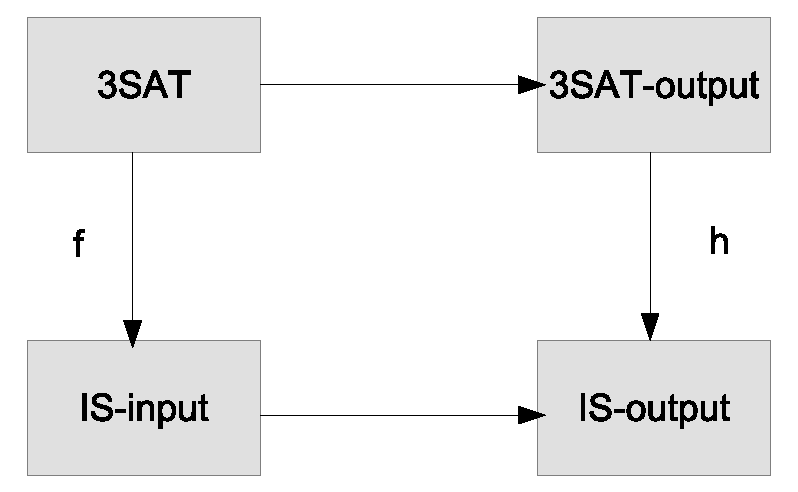
\includegraphics[width=3.0in]{figures/reduction-IS}
\caption{\label{fig:reduction-IS}3SAT and IS reduction}
\end{center}
\end{figure}

In the first step, we prove that the function f takes polynomial time. For each clause, we can get a triangle, and make each variable in the clause be the vertex in the triangle. Then we connect $x_{i}$ with $\overline{x_{i}}$. Thus, we can get a graph which we will be used to max IS. This is a polynomial time operation and Figure~\ref{fig:3SAT-IS} shows the graph we get after the transformation.

Then we can solve the IS problem. We can treat this as a black box. At last, we go to the last step, transform the result from IS to 3SAT with the function h.

In order to prove that if G has a k IS, then 3SAT is satisfiable and if not, then 3SAT is not satisfiable, we prove the controdictory that is if 3SAT is satisfiable we have a k IS and if not, we don not have a k IS.

First, suppose there is an independent set I of size m(where m is the nuber of clauses). Then it must have exactly one vertex from each triangle, since there are m triangles, and having two vertices from the same triangle would violate independence. Let $x_{i} = true$ if at least on $x_{i}$ vertex is in I, $x_{i} = false$ if at least one $\overline{x_{i}}$ is in I, and $x_{i} = true$ if neither condition holds. (The first two conditions cannot both occur for the same $x_{i}$, since we constructed edeges between all contradictory pairs of variables.) By construction, this satisfies $\phi$, because for each clause we have made at least one of the three assignments that will satisfy it.

Conversely, if $\phi$ is satisfiable, pick one of assignments for the varialbes. For each triangle, there is at least one vertex to be true. So for each triangle, there is only one vertex chosen as there are m variables and m triangles. And for the edges by connecting $x_{i}$ and $\overline{x_{i}}$, only one of them is chosen as they are controdictories. So, the graph has a IS with m.

So this proves that $\phi$ can be satisfied if and only if G has an independent set of size m.  

\begin{figure}[bht]
\begin{center}
     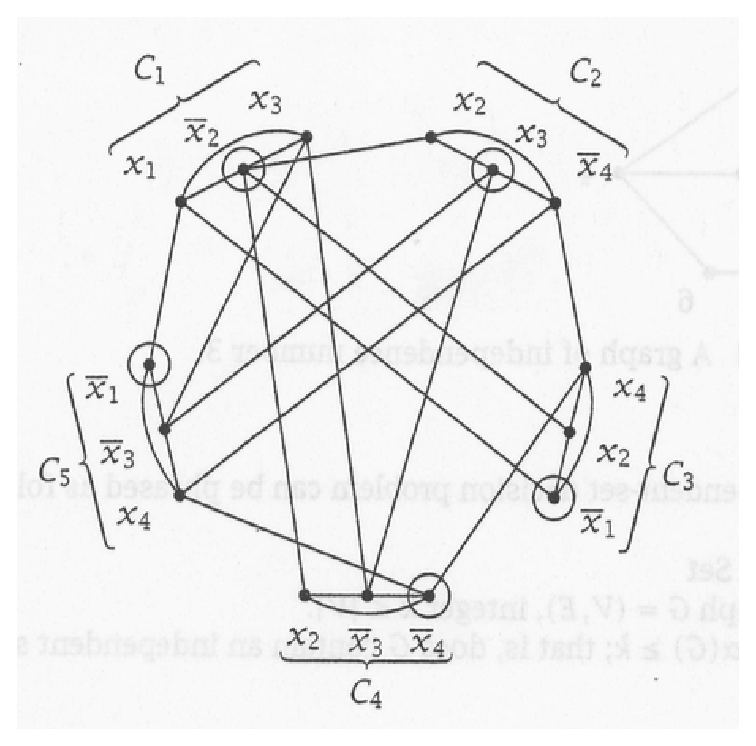
\includegraphics[width=3.0in]{figures/3SAT-IS}
\caption{\label{fig:3SAT-IS}IS graph from 3SAT}
\end{center}
\end{figure}

\section{3SAT $\rightarrow$ Graph Coloring}
K-colorability problem:

Input: G = (V, E), k $\le$ $|V|$.

Question: is $\chi \le$ k? Can v $\in$ V be colored at most k colors such that no adj vertices have a same color?

What we prove is that 3-colorability problem is NPC by reducint 3SAT to it.

Similarly, we have a reduction graph for 3-colorability problem in Figure~\ref{fig:reduction-3C}.

\begin{figure}[bht]
\begin{center}
     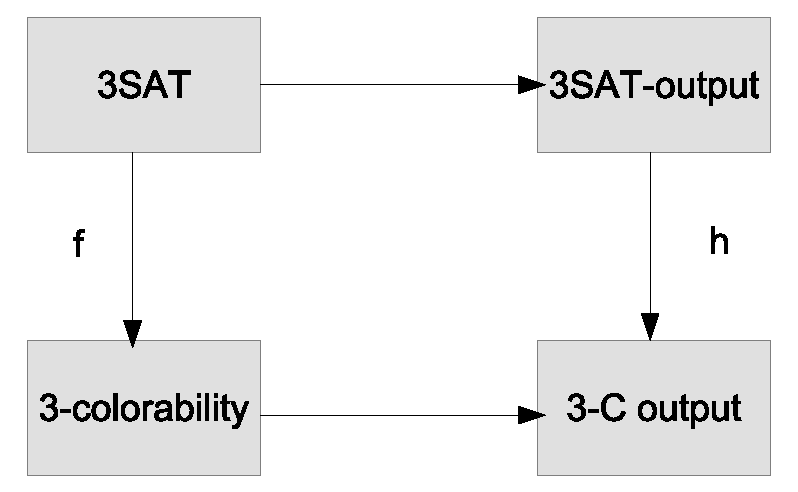
\includegraphics[width=3.0in]{figures/reduction-3C}
\caption{\label{fig:reduction-3C}3SAT and 3-colorability reduction}
\end{center}
\end{figure}

First, we will prove that function f is polynomial.
Before that, we learn about three different Gadget shown in Figure~\ref{fig:gadgets}. 

In the first gadgets, there are three vertices t, f and b denoting color T, F and B. The colors of T and F correspond to true and false, while the third color, the color of B, is used for encoding purposes.

For each variable $x_{i}$ in $\phi$, we get the second gadget. The three vertices are $x_{i}$, $\overline{x_{i}}$ and b.

At last for each clause in $\phi$, we build the third gadget which garantees at least one variable in each clause is satisfied by the coloring. And the six vertices in a row is the baseline of the gadget and the outer two vertices of the baseline are its endpoints. The three labeled vertices are the tops of the triangles.

So with these three gadgets, we can construct a graph G in Figure~\ref{fig:3SAT-3C} (same example in IS). 

This gadget has the key properties that (1) every valid 3-coloring of it has opposite corners the same color and (2) any such coloring of the corners extends to a 3-coloring of the entire gadget. These properties can be shown by enumerating the gadget’s possible 3-colorings.

So the functino f takes polynomial time, and we can solve the 3-colorability using a black box algorithm. And at last, we need to prove that 3SAT is satisfiable if and only if 3-colorability is satisfiable.

\begin{figure}[bht]
\begin{center}
     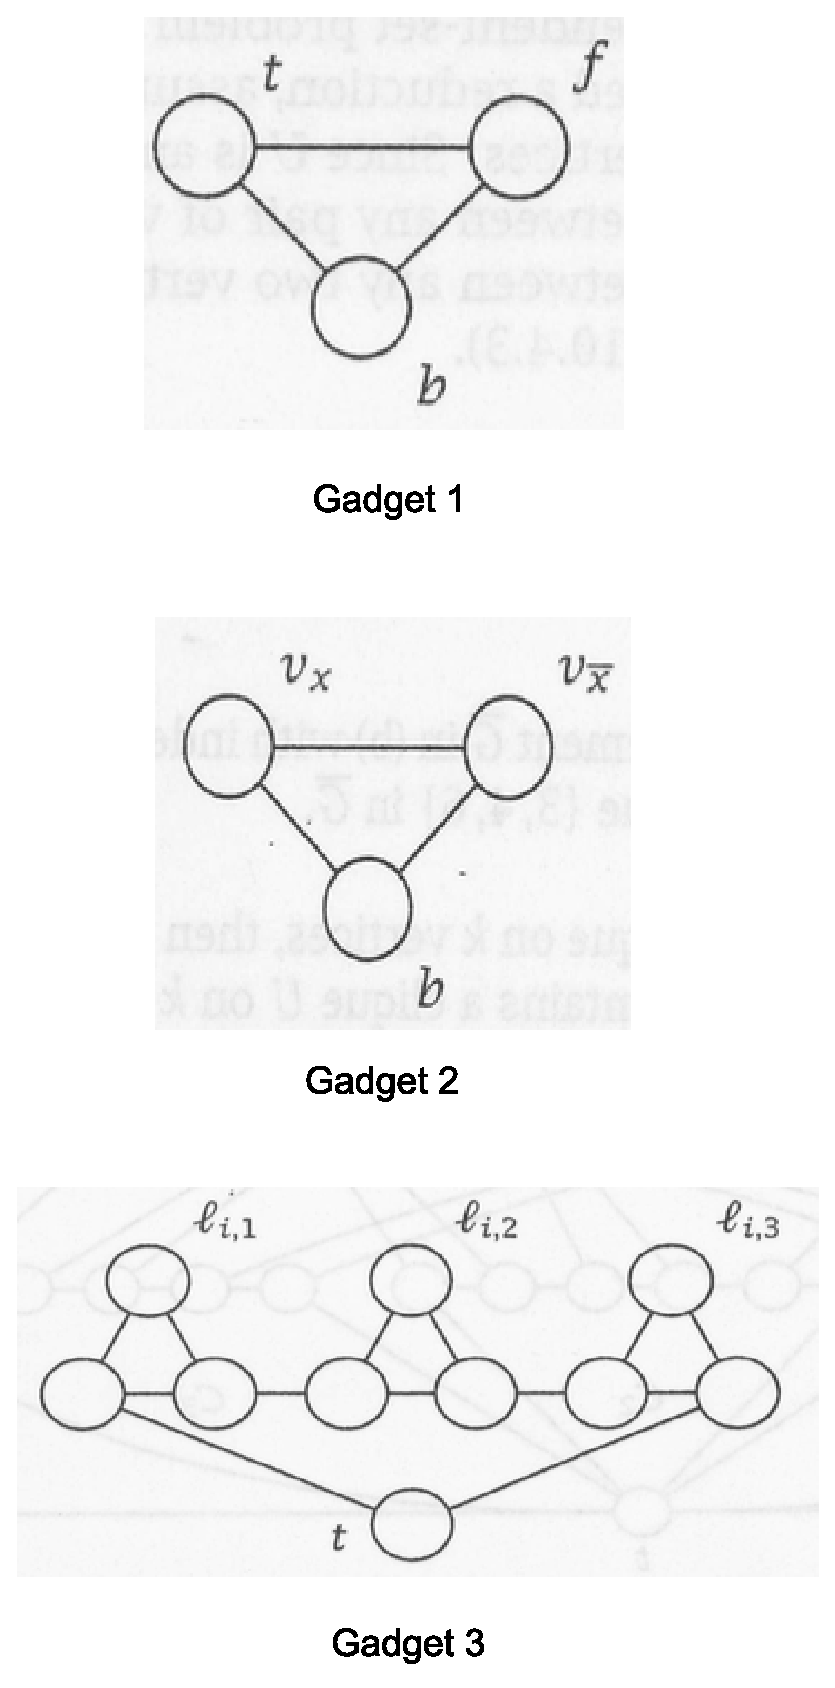
\includegraphics[width=2.5in]{figures/gadgets}
\caption{\label{fig:gadgets}3 different gadgets}
\end{center}
\end{figure}

\begin{figure}[bht]
\begin{center}
     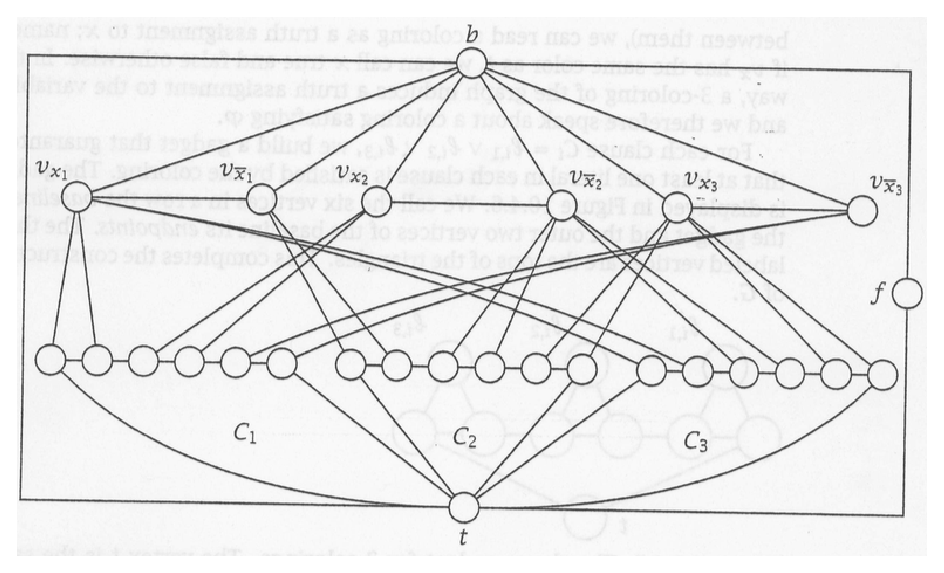
\includegraphics[width=2.5in]{figures/3SAT-3C}
\caption{\label{fig:3SAT-3C}3-colorability graph from 3SAT}
\end{center}
\end{figure}

We first argue that a 3-coloring of G translates to a satisfying assignment
of $\phi$. The vertices t, f , and b have to be colored with the three different
colors T, F and B. $v_{x}$ and $v_{\overline{x}}$ have to be colored T and F, or F and T, because they are conneted with B. Then we can construct that: if $v_{x}$ is T, we let x be true, and false otherwise. Then we need to prove that this assignment satisfies $\phi$. Consider a clause $C_{i}= l_{i,1} \wedge l_{i,2} \wedge l_{i,3}$ and its corresponding gadget. Assume that $l_{i,1}, l_{i,2}$ andl $l_{i,3}$ are all false. Then the tops of all three triangles in the gadgets are F. Then in the baseline, it should be T and B alternatively. Thus one of the endpoints has to be T, which is not possible since it is connected to T.

Hence we get that at least one of these three has to be T. Then $C_{i}$ is satisfied. And as this is true for all clauses, then all clauses can be satisfied and therefore $\phi$ is satisfied. 

Then, we prove that if $\phi$ is satisfiable, then G can be 3-colored. Fix a satisfying assignment of G. Color vertices t, f, and b with colors T, F, and B. T is true and F is false. For each variable x in $\phi$, we get vertex $v_{x}$ T and $v_{\overline{x}}$ F. Finally, we have to show how to color the gadgets. Since we chose a satisfying assignment, at least one of the three top vertices of the triangles has to be T. By figuring out all the different cases for each variable in a clause, we can see that G can be 3-colored. (There are 5 different asymmetric cases.)

\bibliographystyle{abbrv}
\bibliography{0301}

\end{document}
